% ----------------------- TODO ---------------------------
% Diese Daten müssen pro Blatt angepasst werden:
\newcommand{\NUMBER}{1}
\newcommand{\EXERCISES}{3}
% Diese Daten müssen einmalig pro Vorlesung angepasst werden:
\newcommand{\COURSE}{Chip Design}
\newcommand{\BETREUER}{Adrian Frischknecht\\ Julia Grosse}
\newcommand{\STUDENTA}{Luisa Renz}
\newcommand{\STUDENTB}{Lars Wolff}
\newcommand{\STUDENTC}{Felix Lorenz}
\newcommand{\DEADLINE}{15.11.2018}
% ----------------------- TODO ---------------------------

%Template 
\documentclass[a4paper]{scrartcl}
\usepackage[utf8]{inputenc}
\usepackage[ngerman]{babel}
\usepackage{geometry,forloop,fancyhdr,fancybox,lastpage}
\geometry{a4paper,left=3cm, right=3cm, top=3cm, bottom=3cm}

%Math
\usepackage{amsmath,amssymb,tabularx}

%Figures
\usepackage{graphicx,tikz,color,float}
\usetikzlibrary{shapes,trees}

%Algorithms
\usepackage[ruled,linesnumbered]{algorithm2e}

%Kopf- und Fußzeile
\pagestyle {fancy}
\fancyhead[L]{Betreuer: \BETREUER}
\fancyhead[C]{\COURSE}
\fancyhead[R]{\today}

\fancyfoot[L]{}
\fancyfoot[C]{}
\fancyfoot[R]{Seite \thepage}

%Formatierung der Überschrift, hier nichts ändern
\def\header#1#2{
  \begin{center}
    {\Large \textbf{Protokoll #1}}\\
    {(Abgabetermin #2)}
  \end{center}
}

%Definition der Punktetabelle, hier nichts ändern
\newcounter{punktelistectr}
\newcounter{punkte}
\newcommand{\punkteliste}[2]{%
  \setcounter{punkte}{#2}%
  \addtocounter{punkte}{-#1}%
  \stepcounter{punkte}%<-- also punkte = m-n+1 = Anzahl Spalten[1]
  \begin{center}%
  \begin{tabularx}{\linewidth}[]{@{}*{\thepunkte}{>{\centering\arraybackslash} X|}@{}>{\centering\arraybackslash}X}
      \forloop{punktelistectr}{#1}{\value{punktelistectr} < #2 } %
      {%
        \thepunktelistectr &
      }
      #2 &  $\Sigma$ \\
      \hline
      \forloop{punktelistectr}{#1}{\value{punktelistectr} < #2 } %
      {%
        &
      } &\\
      \forloop{punktelistectr}{#1}{\value{punktelistectr} < #2 } %
      {%
        &
      } &\\
    \end{tabularx}
  \end{center}
}

\begin{document}

\begin{tabularx}{\linewidth}{m{0.2 \linewidth}X}
  \begin{minipage}{\linewidth}
    \STUDENTA\\
    \STUDENTB\\
    \STUDENTC
  \end{minipage} & \begin{minipage}{\linewidth}
    \punkteliste{1}{\EXERCISES}
  \end{minipage}\\
\end{tabularx}

\header{Nr. \NUMBER}{\DEADLINE}

% ----------------------- TODO ---------------------------
% Hier werden die Aufgaben/Lösungen eingetragen:

\section*{Aufgabe 1}
Zeichnen Sie anhand der Elementaranweisung (netlist) einen zugehörigen Schaltplan.\\

\section*{Aufgabe 2}
\begin{figure}[H]
\centering
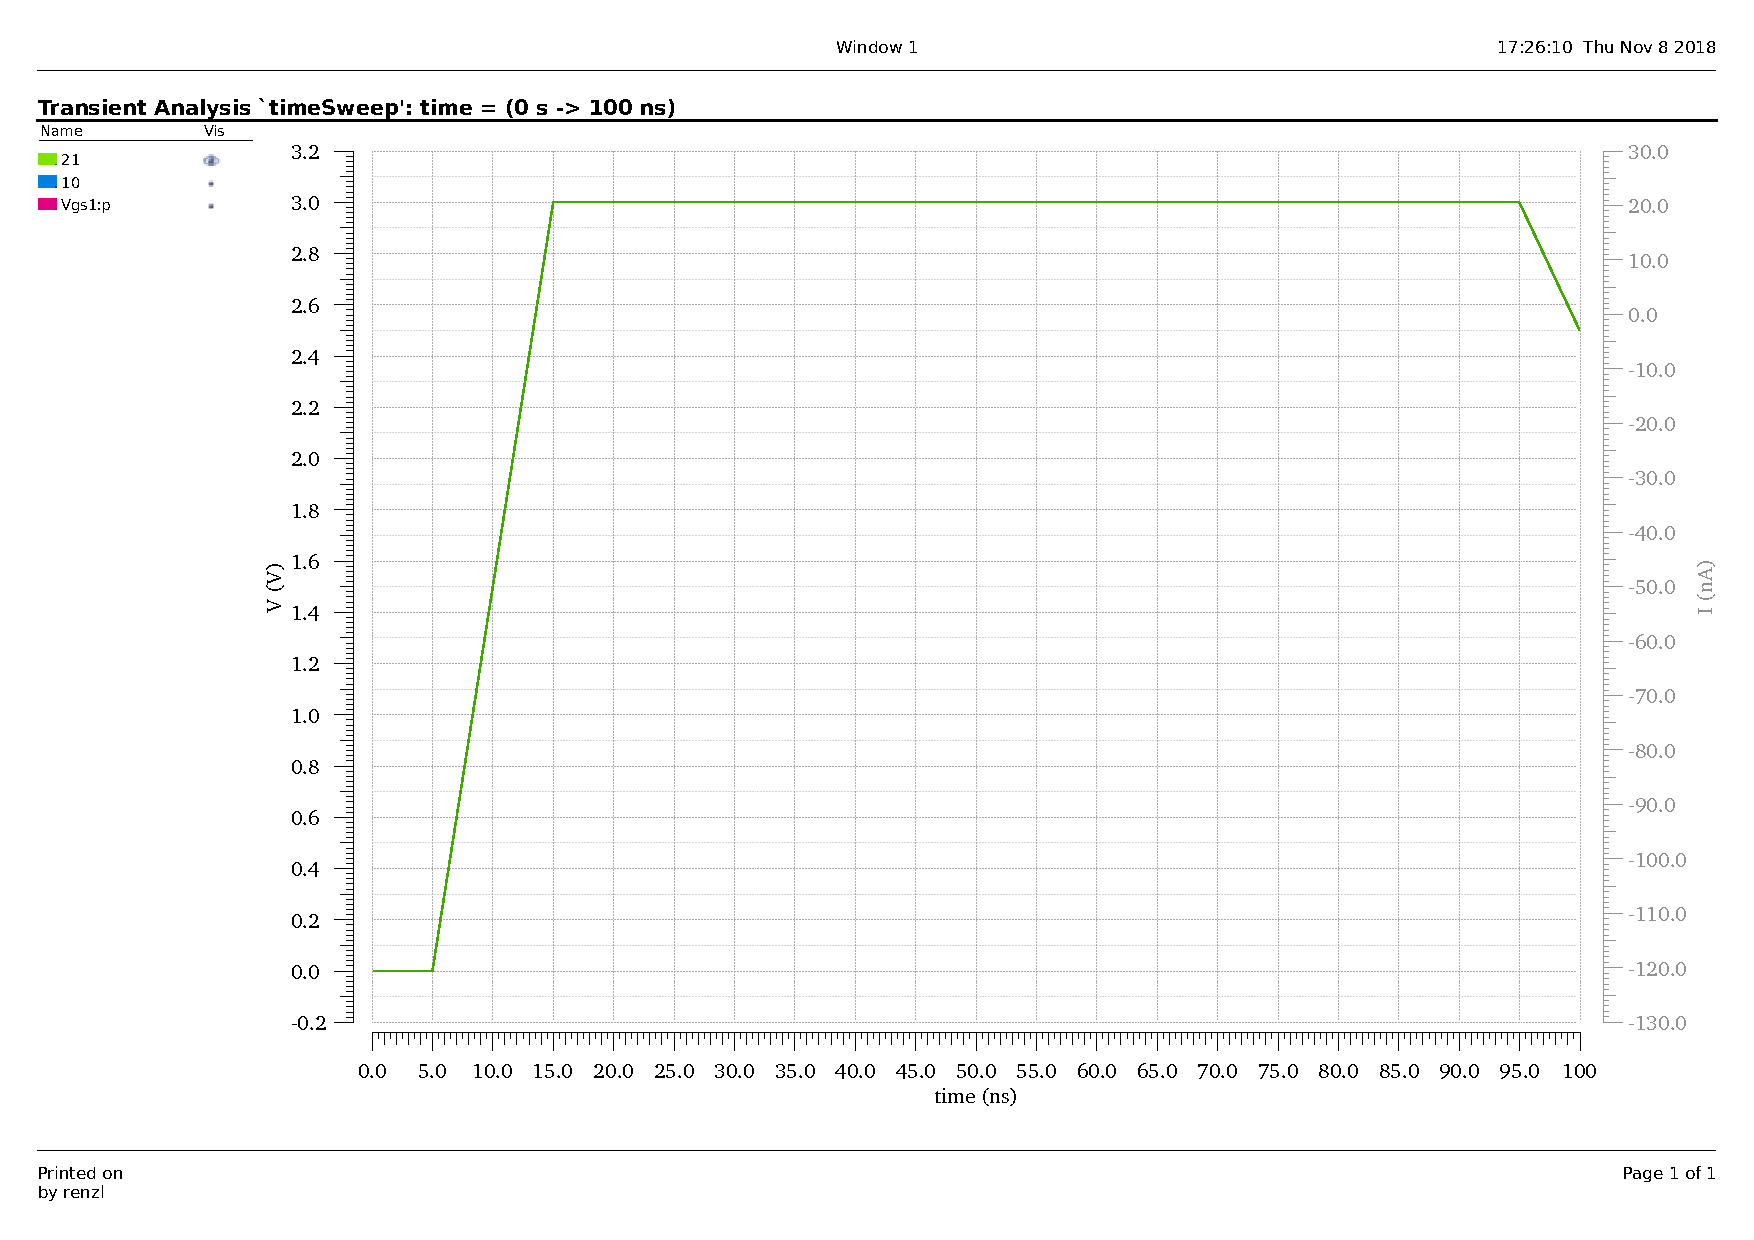
\includegraphics[width=11cm]{print.pdf}
\caption{Spannungsverlauf der Quelle $V_{GS1}$}
\end{figure}
\section*{Aufgabe 3}
\begin{enumerate}
    \item Wofür steht die Abkürzung des Programmnamens SPICE?
\item Erklären Sie kurz in einigen Sätzen was SPICE ist und wofür es verwendet wird.
\item Erklären Sie, was die Steueranweisung .tran bewirkt.
\end{enumerate}

\end{document}
%%% Local Variables:
%%% mode: latex
%%% TeX-master: t
%%% End:
